\chapter{Numerical Time Integration of Partial/Ordinary Differential Equations}

\section{Introduction}

Many engineering problems are described as either a partial differential equation (PDE) or ordinary differential equation (ODE). A broad class of important problems is called the ``Initial Value Problem'' (IVP). Take for example the continuity equation in semiconductors, which is given as\begin{IEEEeqnarray}{rCl}
\frac{\partial n}{\partial t} & = & -\text{div}\left(\bm{J}\right) + G_\text{n} - R_\text{n} \label{eq:continuityEqn}
\end{IEEEeqnarray}where $n$ is the carrier concentration, $\bm{J}$ is the current density flowing through the semiconductor, $G_\text{n}$ and $R_\text{n}$ are the rates of carrier generation and recombination due to generation and recombination processes, respectively. The IVP is as follows. Assume that at time, $t=0$, the carrier concentration is $n(t=0)={0}$ and we want to find the time-dependent profile of the carrier concentration, $n(t)$.

In general, the PDE is more complicated than that in Equation~(\ref{eq:continuityEqn}), and the time derivative or slope function is denoted as $\dot{y}(t)=f(t, y)$, where $y(t)$ is the quantity we are trying to solve for, having the initial condition $y(t=0)=y_{0}$.

\section{The Forward (Explicit) Euler Method}\label{sec:forwardEuler}

One method to obtain $y(t)$ from $f(t,y)$ and $y_{0}$ is to use the forward Euler method. First, the time range over which to determine $y(t)$ is discretized into a uniform grid. The time difference between each grid point, $\Delta t=h$ is called the \emph{time step}. The IVP is solved by calculating $y(t_{n})$ iteratively starting at $t_{n}=0$ and $y(t=0)=y_0$ using the formula\begin{IEEEeqnarray}{rCl}
y(t_{n}+h) & = & y(t_{n}) + hf(t_{n},y(t_{n})) \label{eq:compExEuler}
\end{IEEEeqnarray}Mathematically, the Equation~(\ref{eq:compExEuler}) is unwieldy and we simplify the expression using $t_{n+1}=t_{n}+h$, $y_{n+1}=y(t_{n+1})$ and $y_{n}=y(t_{n})$, which gives\begin{IEEEeqnarray}{rCl}
y_{n+1} & = & y_{n} + hf(t_{n},y_{n}) \label{eq:simpExEuler}
\end{IEEEeqnarray}

\subsection{Example 1: Solutions with Persistent Oscillations}

Consider the function $y(t) = \sin (t)$ and its time derivative, $\dot{y}(t) = \cos (t)$. The numerical solution for different time steps are plotted in Fig.~\ref{fig:IVP1}. As clearly seen, the error reduces with the size of the time step---a smaller time step returns a numerical result that is closer to the ideal solution.

\subsection{Example 2: Solutions with Damped Relaxations}

Another commonly observed function is $y(t) = \exp(-t)$ and its time derivative, $\dot{y}(t) = -\exp(-t)$. The numerical solution for different time steps are plotted in Fig.~\ref{fig:IVP2}. As clearly seen, the error also reduces with the size of the time step.\afterpage{
\begin{figure}[!t]
\centering
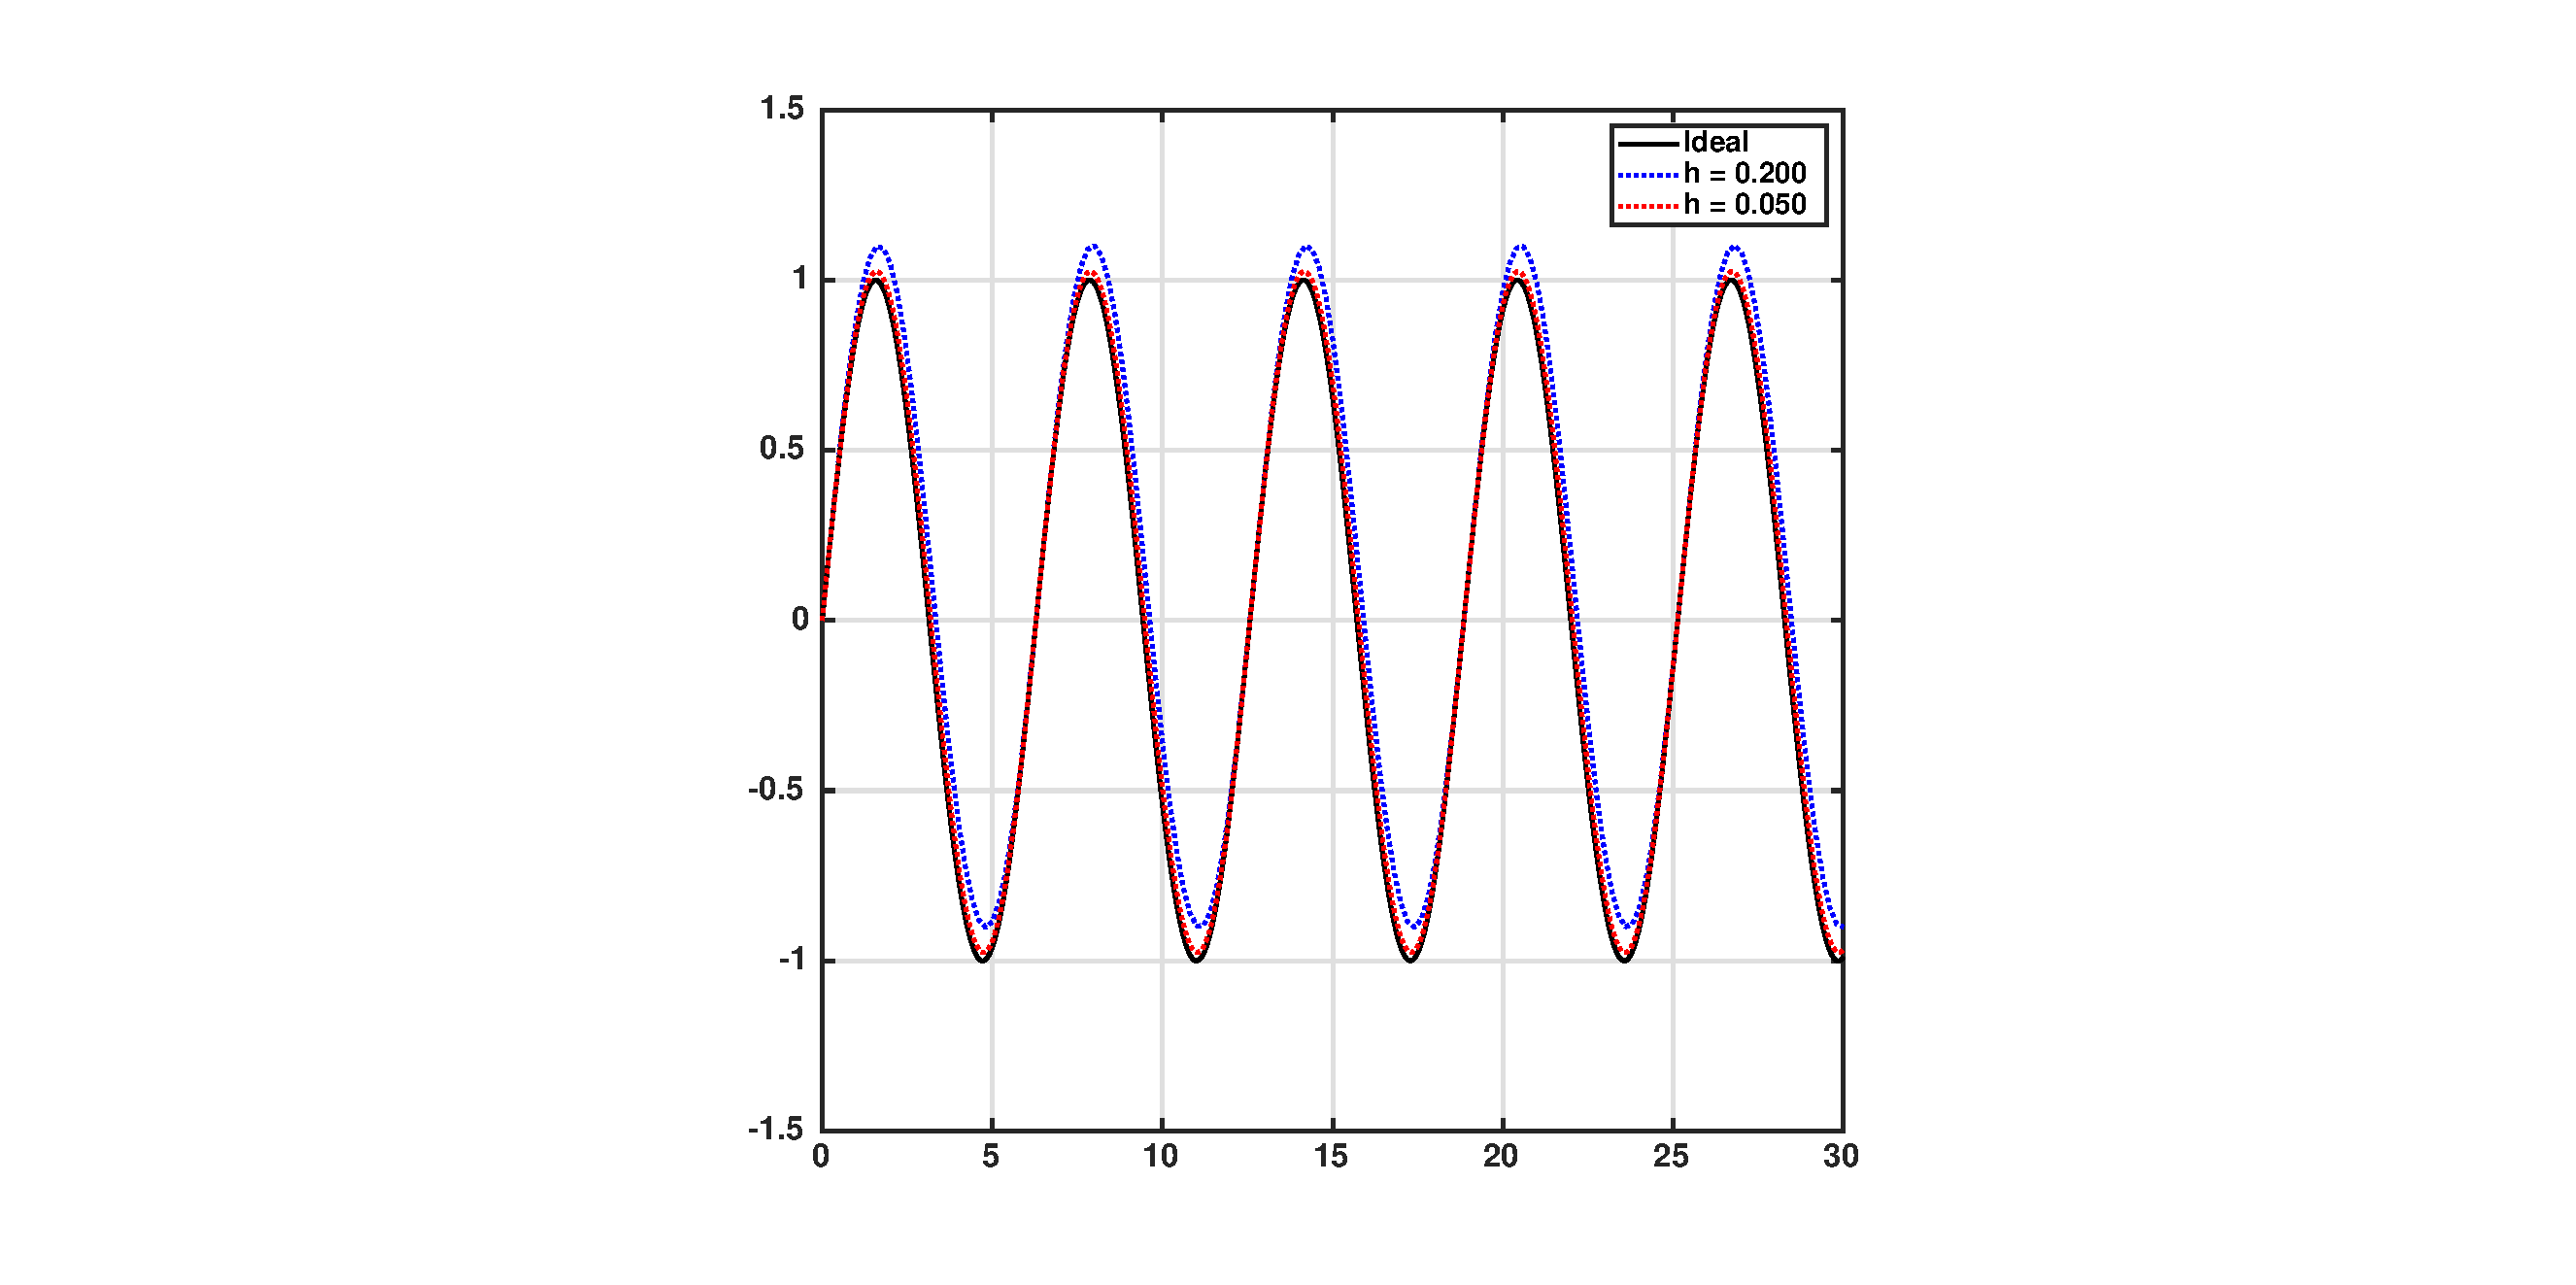
\includegraphics[scale=0.4]{ResearchNotes_TimePDE/figs/eulerTest.eps}
\caption{Numerical solution for the IVP with $\dot{y}(t)=\cos(t)$ and $y_{0}=0$ for different step sizes as compared to the ideal solution $y(t)=\sin(t)$.}
\label{fig:IVP1}
\end{figure}\begin{figure}[!t]
\centering
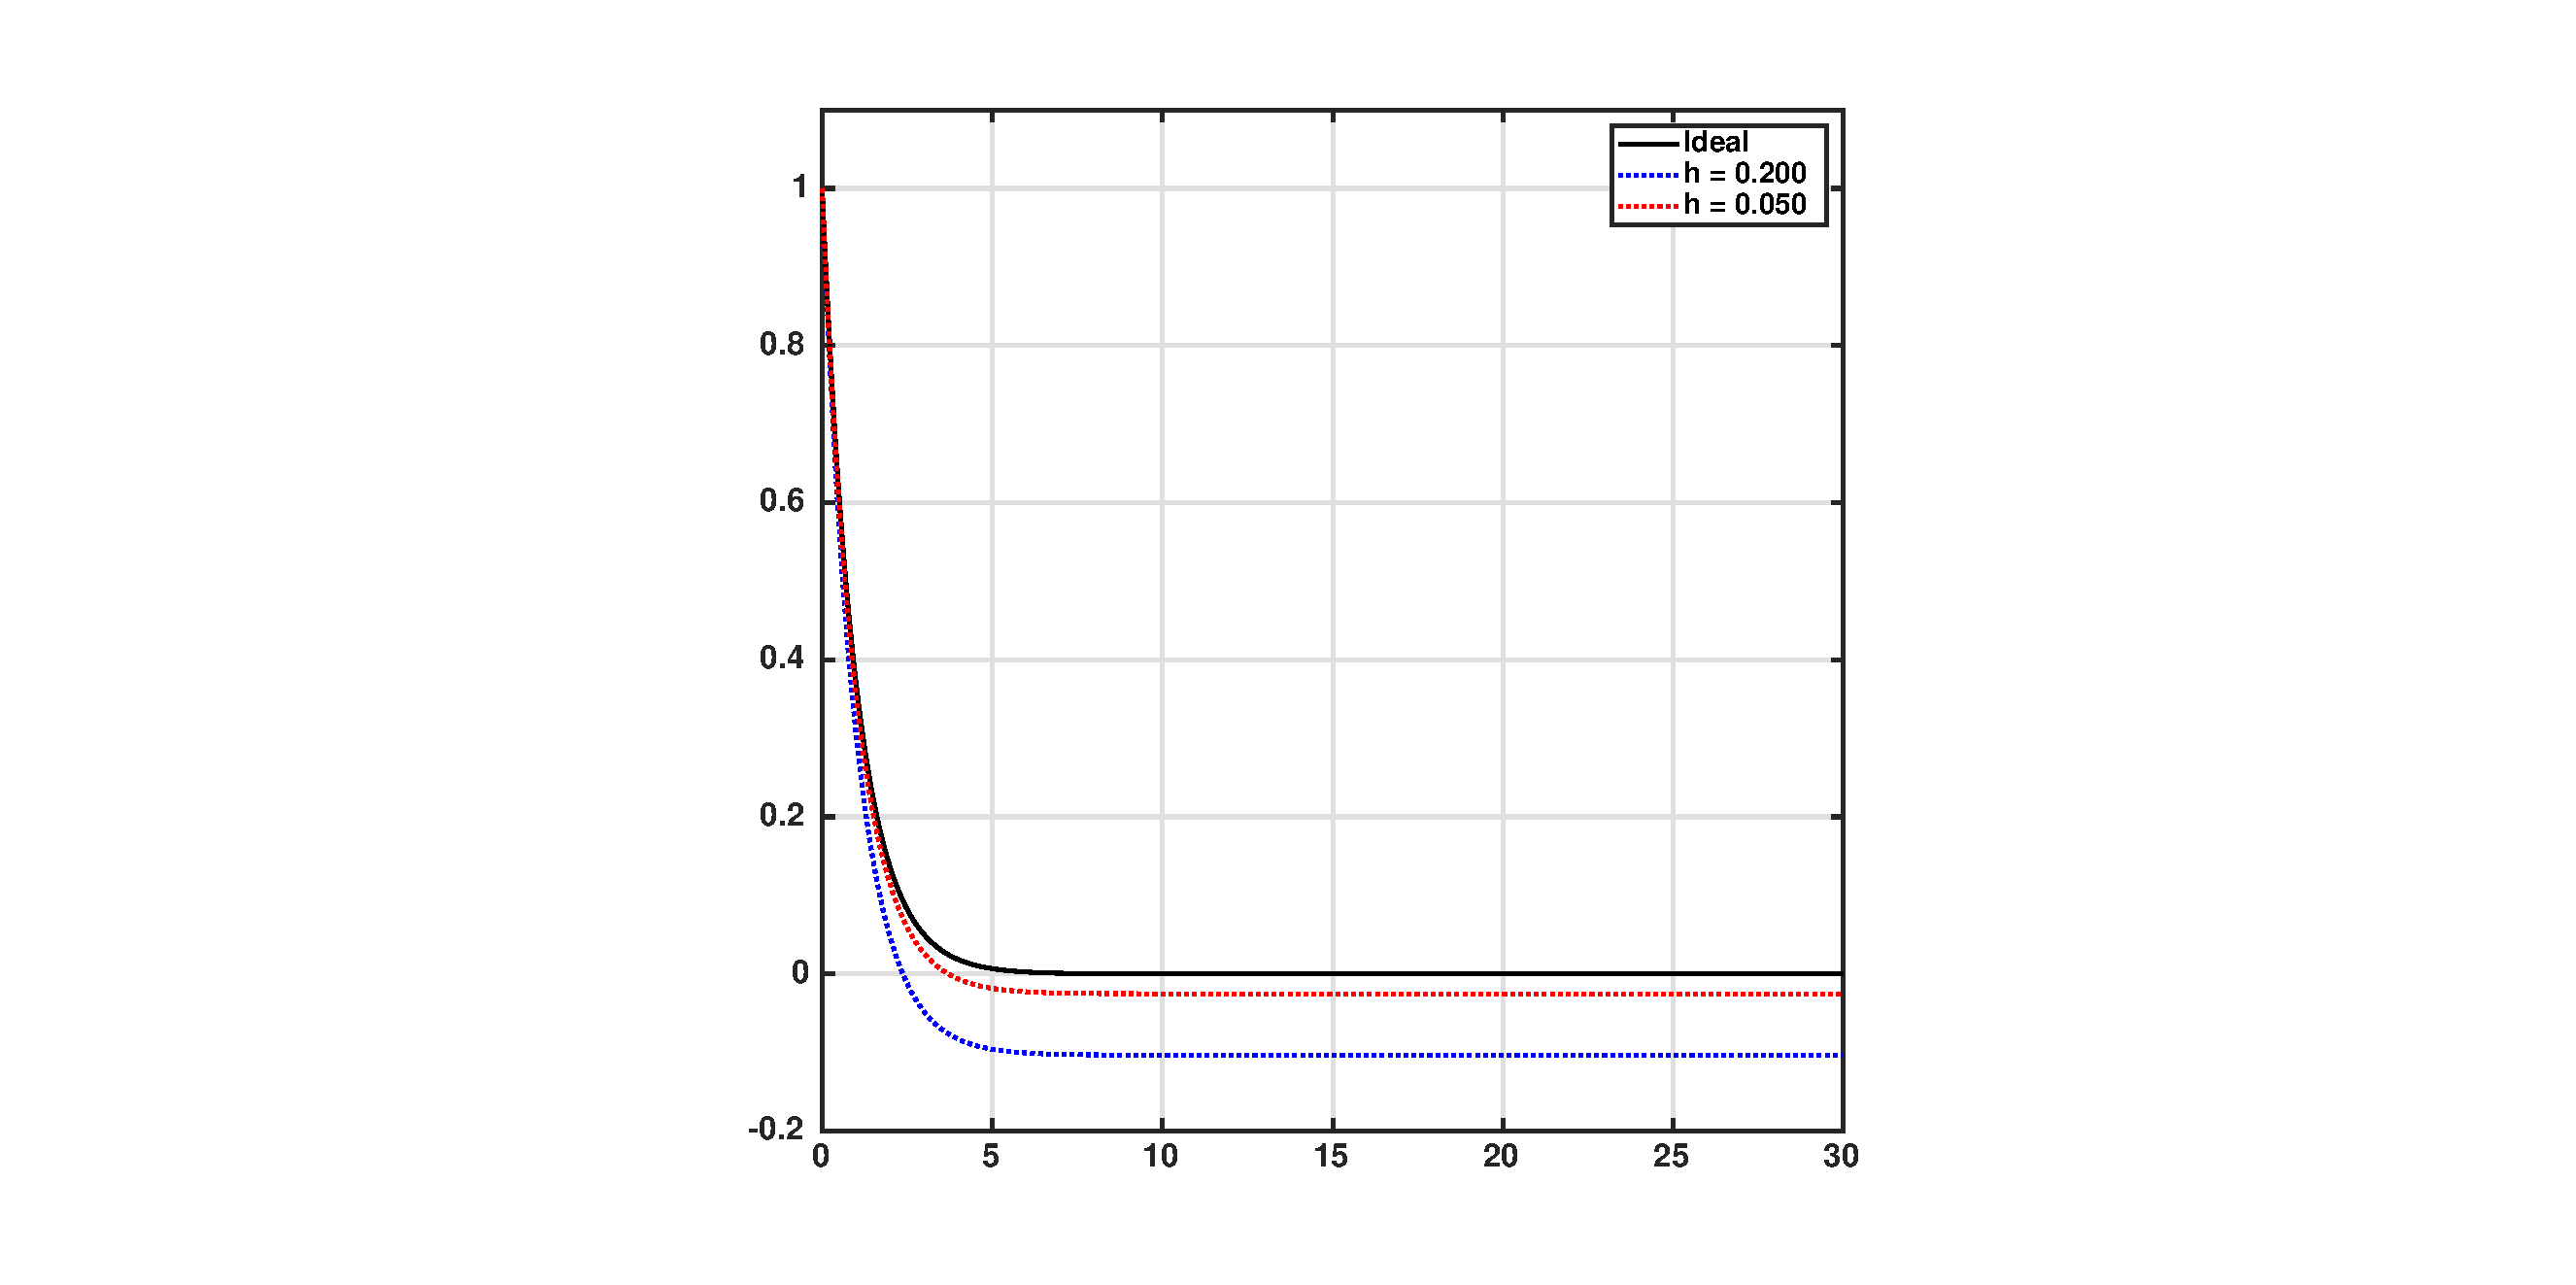
\includegraphics[scale=0.4]{ResearchNotes_TimePDE/figs/eulerTest2.eps}
\caption{Numerical solution for the IVP with $\dot{y}(t)=-\exp(-t)$ and $y_{0}=1.0$ for different step sizes as compared to the ideal solution $y(t)=\exp(-t)$.}
\label{fig:IVP2}
\end{figure}\clearpage
}

In Equation~(\ref{eq:simpExEuler}), $y_{n+1}$ appears only on the LHS, which means it is \emph{explicitly} defined. Thus, the forward Euler method is an explicit method. In contrast, the \emph{backward} (\emph{implicit}) Euler method is described by\begin{IEEEeqnarray}{rCl}
y_{n+1} & = & y_{n} + hf(t_{n+1},y_{n+1}) \label{eq:compImEuler}
\end{IEEEeqnarray}Furthermore, the Euler methods calculate $y_{n+1}$ using only $y_{n}$ and not previous $y$ values (\emph{i.e.}, $y_{n-1}$, $y_{n-2}$, etc.). Hence, the Euler methods are examples of \emph{single step methods}. The Adams-Bashforth methods, Adams-Moulton methods and the backward differentiation formulas (BDF) are \emph{linear multistep methods}. For example, the two-step Adams-Bashforth method is described by the formula\begin{IEEEeqnarray}{rCl}
y_{n+2} & = & y_{n+1} + \frac{3}{2}hf(t_{n+1},y_{n+1}) - \frac{1}{2}hf(t_{n},y_{n}) \label{eq:AB12}
\end{IEEEeqnarray}where information at $y_{n}$ is used to calculate $y_{n+2}$ from $y_{n+1}$. Consequently, linear multistep methods need to be initialized in order to proceed.

\section{Higher Order Explicit Methods}

Equation~(\ref{eq:simpExEuler}) has a similar form as the power series expansion, which is written as\begin{IEEEeqnarray}{rCl}
y(t_{n+1}) & = & \sum^{+\infty}_{i=0}a_{i}y^{(i)}(t_{n})
\end{IEEEeqnarray}where the superscript in $y^{(i)}$ denotes the $i$-th derivative of $y$. Thus, the forward Euler method may be thought of as a first order estimation for $y(t_{n+1})$ and the full expression of Equation~(\ref{eq:simpExEuler}) is\begin{IEEEeqnarray}{rCl}
y_{n+1} & = & y_{n} + hf(t_{n},y_{n}) + \mathcal{O}(h^{2})
\end{IEEEeqnarray}and the error in using Equation~(\ref{eq:simpExEuler}) to approximate $y(t)$ is $\mathcal{O}(h^{2})$. By expanding the power series further, we can derive higher order explicit methods for $y_{n+1}$ and reduce the error.

\subsection{The Heun Method}

The Heun method is a second order method to approximate $y_{n+1}$ and is given by the expression\begin{IEEEeqnarray}{rCl}
y_{n+1} & = & y_{n} + h\frac{k_{1}+k_{2}}{2},~\text{where} \label{eq:heun} \\
k_{1} & = & f(t_{n},y_{n}) \nonumber \\
k_{2} & = & f(t_{n+1},y_{n}+hk_{1}) \nonumber
\end{IEEEeqnarray}It can be seen that $y_{n+1}$ is determined using two evaluations of $f()$ ($k_{1}$ and $k_{2}$). The evaluation of $k_{1}$ is akin to the explicit Euler method. The evaluation of $k_{2}$ occurs at the point predicted using the Euler method. The average of $k_{1}$ and $k_{2}$ is then used to estimate $y_{n+1}$.

\subsection{The 4-th Order Runge-Kutta (RK) Method}

German mathematicians Carl Runge and Wilhelm Kutta derived methods (also called Runge-Kutta methods or RK methods) to approximate $y_{n+1}$. The 4-th order RK method (RK4) is given by the expression\begin{IEEEeqnarray}{rCl}
y_{n+1} & = & y_{n} + \frac{h}{6}\left(k_{1}+2k_{2}+2k_{3}+k_{4}\right),~\text{where} \\
k_{1} & = & f(t_{n},y_{n}) \nonumber \\
k_{2} & = & f\left(t_{n}+\frac{h}{2}, y_{n}+h\frac{k_{1}}{2}\right) \nonumber \\
k_{3} & = & f\left(t_{n}+\frac{h}{2}, y_{n}+h\frac{k_{2}}{2}\right) \nonumber \\
k_{4} & = & f(t_{n+1},y_{n}+hk_{3}) \nonumber
\end{IEEEeqnarray}In this method $f()$ are evaluated at points within the time step to obtain a better approximation of $y_{n+1}$.

\subsection{The Butcher Tableau}

From the methods discussed so far, it can be seen that the general equation for determining $y_{n+1}$ in single step methods is \begin{IEEEeqnarray}{rCl}
y_{n+1} & = & y_{n} + h\sum^{s}_{i=1}b_{i}k_{i},~\text{where} \\
k_{1} & = & f(t_{n},y_{n}) \nonumber \\
k_{2} & = & f(t_{n}+c_{2}h,y_{n}+ha_{21}k_{1}) \nonumber \\
k_{3} & = & f(t_{n}+c_{3}h,y_{n}+ha_{31}k_{1}+ha_{32}k_{2}) \nonumber \\
& \vdots & \\
k_{s} & = & f(t_{n}+c_{s}h, y_{n}+h\sum^{s-1}_{j=1}a_{s,j}k_{j}) \nonumber
\end{IEEEeqnarray}where $k_{i}$ is calculated in the $i$-th stage of the method. The mathematician John C. Butcher proposed a concise way of describing the numerical methods using a tableau called the \emph{Butcher tableau} (see Fig.~\ref{fig:butcherTab}).

From the earlier examples, we can see that the Butcher tableaus for the Euler method and RK4 method are given by Figs.~\ref{fig:eulerButcher} and Fig.~\ref{fig:rk4Butcher}. The Heun method is a special case of a more general method called the \emph{midpoint method}, which has the Butcher tableau given in Fig.~\ref{fig:midpointButcher}.

\begin{figure}[!b]
\centering
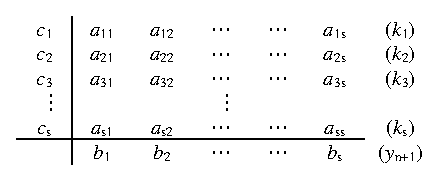
\includegraphics[scale=1.0]{ResearchNotes_TimePDE/figs/ButcherTableau.eps}
\caption{The general form of a Butcher Tableau}
\label{fig:butcherTab}
\end{figure}
\begin{figure}[!b]
\centering

\includegraphics[scale=1.0]{ResearchNotes_TimePDE/figs/eulerButcher.eps}
\caption{Butcher Tableau for the Euler method.}
\label{fig:eulerButcher}
\end{figure}
\begin{figure}[!b]
\centering
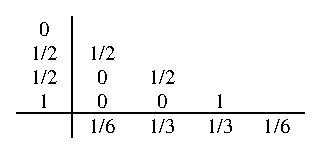
\includegraphics[scale=1.0]{ResearchNotes_TimePDE/figs/rk4Butcher.eps}
\caption{Butcher Tableau for the RK4 method.}
\label{fig:rk4Butcher}are
\end{figure}
\begin{figure}[!b]
\centering
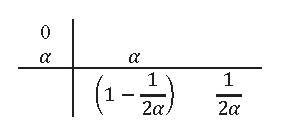
\includegraphics[scale=1.0]{ResearchNotes_TimePDE/figs/midpointTableau.eps}
\caption{Butcher Tableau for the midpoint method. The Heun method is the case where $\alpha=1$.}
\label{fig:midpointButcher}
\end{figure}

The algorithm for executing the explicit methods is shown in Algorithm~\ref{algo:algo1}.
\begin{algorithm}[H]
\caption{Numerical method to solve IVP without adaptive time stepping}
\label{algo:algo1}
\hspace*{\algorithmicindent} $\textbf{Inputs:}~a_{i,j},~b_{i}~\text{and}~c_{i}~\text{from Butcher tableau,}~f(t,y),~t_\text{end},~h_\text{init},~\text{and}~y_{0}$ \\
\hspace*{\algorithmicindent} $\textbf{Outputs:}~y~\text{for all discrete time points,~}t\in{}[0,~t_\text{end}] $
\begin{algorithmic}[1]
\State $n \gets 0$
\State $t_{n} \gets 0$
\State $y_{n} \gets y_{0}$
\State $h_{n} \gets h_\text{init}$
\While{$t_{n} < t_\text{end}$}
  \If{$t_\text{end} < t_{n} + h_{n}$}
    \State $h_{n} = t_\text{end} - t_{n}$
  \EndIf
  \State $k_{1} \gets f(t_{n}, y_{n})$
  \State $\delta{}y \gets b_{1}k_{1}$
  \For{$i0 \gets 2$, number of stages defined in the Butcher tableau}
    \State $t_\text{int} \gets t_{n} + c_{i0}h_{n}$
    \State $j \gets$ number of substeps in stage~$i0$
    \State $y_\text{int} \gets y_{n} + h_{n}\sum^{j}_{i1=1}a_{i0,i1}k_{i1}$
    \State $k_{i0} \gets f(t_\text{int},y_\text{int})$
    \State $\delta{}y \gets \delta{}y + b_{i0}k_{i0}$
  \EndFor
  \State $y_{n+1} \gets y_{n} + h_{n}\cdot\delta{}y$
  \State $t_{n+1} \gets t_{n} + h_{n}$
  \State $n \gets n+1$
\EndWhile
\end{algorithmic}
\end{algorithm}

\afterpage{
\begin{figure}[H]
\centering
\begin{minipage}{0.45\linewidth}
\centering
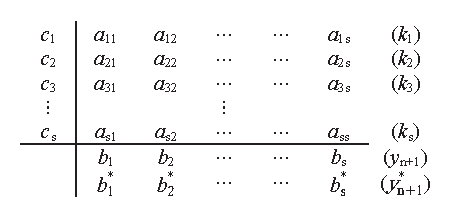
\includegraphics[scale=1.0]{ResearchNotes_TimePDE/figs/EmbeddedButcherTableau.eps}
\caption{The general Butcher tableau for embedded methods.}
\label{fig:embeddedButcher}
\end{minipage}
\quad\quad
\begin{minipage}{0.45\linewidth}
\centering
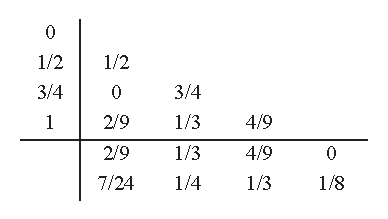
\includegraphics[scale=1.0]{ResearchNotes_TimePDE/figs/rk23.eps}
\caption{The Butcher tableau for the Bogacki-Shampine method. The method has a second order predictor and third order corrector and the LTE is $\bm{O}(h^{3})$.}
\label{fig:rk23}
\end{minipage}
\end{figure}
\begin{figure}[H]
\centering
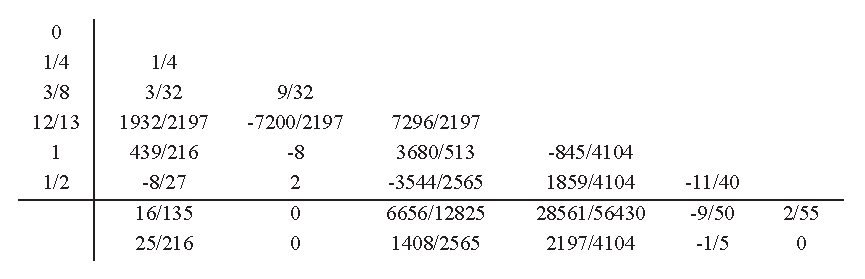
\includegraphics[scale=0.8]{ResearchNotes_TimePDE/figs/fehlberg.eps}
\caption{The Butcher tableau for the Fehlberg method. The method has a fourth order predictor and fifth order corrector and the LTE is $\bm{O}(h^{5})$.}
\label{fig:fehlberg}
\end{figure}\begin{figure}[H]
\centering
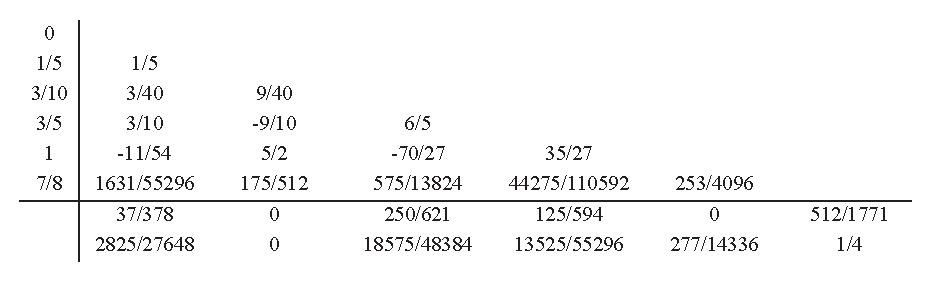
\includegraphics[scale=0.8]{ResearchNotes_TimePDE/figs/rk45ck.eps}
\caption{The Butcher tableau for the Cash-Karp method. The method has a fourth order predictor and fifth order corrector and the LTE is $\bm{O}(h^{5})$.}
\label{fig:rk45ck}
\end{figure}\begin{figure}[H]
\centering
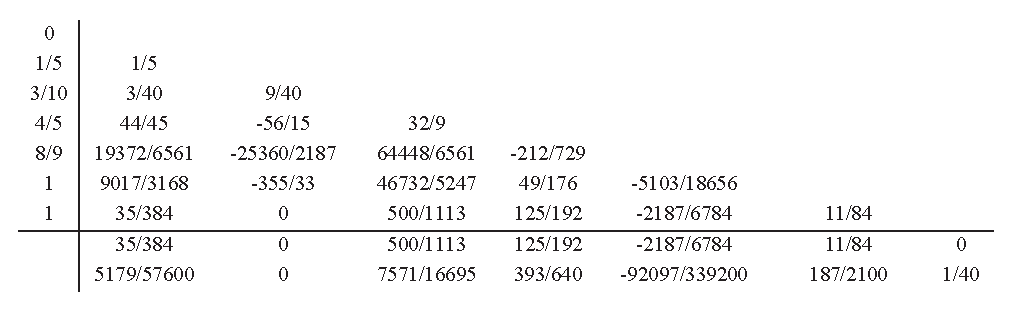
\includegraphics[scale=0.8]{ResearchNotes_TimePDE/figs/rk45dp.eps}
\caption{The Butcher tableau for the Dormand-Prince method. The method has a fourth order predictor and fifth order corrector and the LTE is $\bm{O}(h^{5})$.}
\label{fig:rk45dp}
\end{figure}\clearpage
}

\section{Adaptive time stepping}

As can be seen in Figs.~\ref{fig:IVP1} and \ref{fig:IVP2}, there is a dependence of the accuracy of the solution returned by the numerical method and the time step used. In engineering simulations, the simulation runtime may be reduced if the time steps can be optimized. Adaptive time stepping algorithms attempt to optimize the time step used by ensuring that the estimated local truncation error (\emph{LTE}) is bounded to some tolerance value. The LTE is calculated by subtracting two approximations of $y_{n+1}$---one with order $p$ and another with order $p-1$, which leads to the LTE having order $p$. These methods are sometimes called \emph{predictor-corrector} methods, since one expression gives a low order predicted value of $y_{n+1}$ and the LTE gives a high order corrector to the predictor.

A family of embedded RK methods exist that is computationally efficient in calculating $y_{n+1}$ and the LTE at the $n$-th step, $\bm{\widehat{r}}_{n}$. These methods are computationally efficient because they reduce the number of calls to evaluate $f()$, which is the most computationally intensive portion of the numerical method. Fig.~\ref{fig:embeddedButcher} shows the general form of the Butcher tableau for an embedded method.

Some commonly used embedded explicit methods are those by Bogacki-Shampine (RK23) \cite{Bogacki1989} (Fig.~\ref{fig:rk23}), Fehlberg (RK45F) \cite{Fehlberg1970} (Fig.~\ref{fig:fehlberg}), Cash-Karp (RF45CK) \cite{Cash1990} (Fig.~\ref{fig:rk45ck}), and Dormand-Prince (RK45DP) \cite{Dormand1980} (Fig.~\ref{fig:rk45dp}). A key difference between the RK45 methods is the number of evaluations of $f()$ needed to estimate $y_{n+1}$. Some methods (such as RK23 and RK45DP) have a ``first same as last'' (FSAL) property, which means the predictor is calculated at the last stage.

Adaptive time stepping is performed by calculating the ratio of an error tolerance to the LTE. The next time step in the numerical method is then scaled according to the equation\begin{IEEEeqnarray}{rCl}
h_{n+1} & = & 0.9 \times h_{n} \times \min\left(\max \left(\left(\frac{\text{tol}}{|\bm{\widehat{r}}_{n}|}\right)^{1/(p+1)},0.3\right), 2\right)\label{eq:adapH0}
\end{IEEEeqnarray}where $p$ is the order of the corrector. The factor of 0.9 is a safety factor to limit the change in $h$ and reduce the risk that $h_{n+1}$ is rejected when calculating $y_{n+2}$. The $\min$ and $\max$ further limit $h_{n+1}$ to the range $[0.27h_{n}, 1.8h_{n}]$.

An alternative scheme was proposed by K. Gustafsson in \cite{Gustafsson1988}. The work is motivated by control theory and seeks to handle issues that arise when solving stiff problems (see Section~\ref{subsec:stabilityExp}) and remain useful for both explicit and the implicit methods (to be discussed after Section~\ref{subsec:stabilityExp}). First, Equation~(\ref{eq:adapH0}) is rewritten as\begin{IEEEeqnarray}{rCl}
h_{n+1} & = & \theta{}h_{n} \label{eq:adapH1} \\
\theta & = & \gamma\left(\frac{\text{tol}}{|\bm{\widehat{r}}_{n}|/h_{n}}\right)^{1/p} = \left(\frac{\gamma^{p}\cdot\text{tol}}{|\bm{\widehat{r}}_{n}|/h_{n}}\right)^{1/p}
\end{IEEEeqnarray}where $\gamma$ is the safety factor ($\gamma=0.9$ in Equation~(\ref{eq:adapH0})), and $|\bm{\widehat{r}}_{n}|\propto{}h_{n}$. Taking the $\log()$ on both sides gives\begin{IEEEeqnarray}{rCl}
\log(h_{n+1}) & = & \log(h_{n}) + \frac{1}{p}\left(\log(\gamma^{p}\cdot\text{tol}) - \log\left(\frac{|\bm{\widehat{r}}_{n}|}{h_{n}}\right)\right)
\end{IEEEeqnarray}In \cite{Gustafsson1988}, $\gamma=1.0$ and,\begin{IEEEeqnarray}{rCl}
e_{n} & = &  \log(\gamma^{p}\cdot\text{tol}) - \log\left(\frac{|\bm{\widehat{r}}_{n}|}{h_{n}}\right) \\
P_{n} & = & K_\text{P}\cdot e_{n} \\
I_\text{temp} & = & I_{n-1} + K_\text{I}\cdot{}e_{n} \\
h_\text{temp} & = & \exp\left(P_{n}+I_\text{temp}\right) \\
h_{n+1} & = & \min\left(h_\text{temp},\theta_\text{max}h_{n}\right) \\
I_{n} & = & I_\text{temp} + \log(h_{n+1}) - \log(h_{n})
\end{IEEEeqnarray}where $\theta_\text{max}$ limits the growth of $h$. Then, the time stepping algorithm calculates the following\begin{IEEEeqnarray}{rCl}
h_\text{temp} & = & \left(\frac{\text{tol}}{|\bm{\widehat{r}}_{n}|/h_{n}}\right)^{K_\text{I}}\left(\frac{|\bm{\widehat{r}}_{n-1}|/h_{n-1}}{|\bm{\widehat{r}}_{n}|/h_{n}}\right)^{K_\text{P}}h_{n} \label{eq:gustafTrack} \\
h_{n+1} & = & \min\left(h_\text{temp},\theta_\text{max}h_{n}\right)
\end{IEEEeqnarray}where it is recommended that $\theta_\text{max}=2.0$. Equation~(\ref{eq:gustafTrack}) states that during the execution of the algorithm, $|\bm{\widehat{r}}_{n}|/h_{n}$ needs to be saved for the next time step for adaptive time stepping. Furthermore, two sets of parameters are recommended depending on whether the time step is rejected (\emph{e.g.}, $|\bm{\widehat{r}}_{n}|/h_{n}>1.2\cdot{}\text{tol}$) or accepted. If the time step is accepted, use $K_\text{P}=0.13$ and $K_\text{I}=1/15$. Otherwise, use $K_\text{P}=0$ and $K_\text{I}=1/5$.

The algorithm for executing the explicit methods with adaptive time stepping is shown in Algorithm~\ref{algo:algo2}, where the function, $adaptH()$, can implement either the conventional method, or the Gustafsson method. \begin{algorithm}[H]
\caption{Numerical method to solve IVP with adaptive time stepping}
\label{algo:algo2}
\hspace*{\algorithmicindent} $\textbf{Inputs:}~p\text{~(order of embedded corrector)},~a_{i,j},~b_{i},~b^{*}_{i}~\text{and}~c_{i}~\text{from Butcher tableau,}~f(t,y),~errTol,$ \\
\hspace*{\algorithmicindent}\hspace*{\algorithmicindent}$adaptH(),~t_\text{end},~h_\text{init},~\text{and}~y_{0}$ \\
\hspace*{\algorithmicindent} $\textbf{Outputs:}~y~\text{for all discrete time points,~}t\in{}[0,~t_\text{end}] $
\begin{algorithmic}[1]
\State $n \gets 0$
\State $t_{n} \gets 0$
\State $y_{n} \gets y_{0}$
\State $h_{n} \gets h_\text{init}$
\While{$t_{n} < t_\text{end}$}
  \If{$t_\text{end} < t_{n} + h_{n}$}
    \State $h_{n} = t_\text{end} - t_{n}$
  \EndIf
  \State $rejectH \gets true$
  \While{$rejectH$~is~$true$}
    \State $k_{1} \gets f(t_{n}, y_{n})$
    \State $\delta{}y \gets b_{1}k_{1}$
    \State $LTE_{n} \gets (b_{1} - b^{*}_{1})k_{1}$
    \For{$i0 \gets 2$, number of stages defined in the Butcher tableau}
      \State $t_\text{int} \gets t_{n} + c_{i0}h_{n}$
      \State $j \gets$ number of substeps in stage~$i0$
      \State $y_\text{int} \gets y_{n} + h_{n}\sum^{j}_{i1=1}a_{i0,i1}k_{i1}$
      \State $k_{i0} \gets f(t_\text{int},y_\text{int})$
      \State $\delta{}y \gets \delta{}y + b_{i0}k_{i0}$
      \State $LTE_{n} \gets LTE_{n} + (b_{i0} - b^{*}_{i0})k_{i0}$
    \EndFor
    \State $rejectH, h_\text{recommend} \gets adaptH(p, h_{n}, errTol, LTE_{n}, \delta{}y)$
    \If{$rejectH$ is $true$}
      \State $h_{n} \gets h_\text{recommend}$
    \Else
      \State $h_{n+1} \gets h_\text{recommend}$
    \EndIf
  \EndWhile
  \State $y_{n+1} \gets y_{n} + h_{n}\cdot\delta{}y$
  \State $t_{n+1} \gets t_{n} + h_{n}$
  \State $n \gets n+1$
\EndWhile
\end{algorithmic}
\end{algorithm}

\subsection{Stability of Explicit Methods and Stiffness of IVP}\label{subsec:stabilityExp}

A major disadvantage of explicit methods is that the errors introduced when used to solve stiff IVPs can be extremely large. Examples of stiff problems are encountered when critically damped and overdamped systems are studied. Consider the example of a non-ideal voltage source charging a fixed capacitor, $C_\text{L}$, through an output resistance, $R_\text{out}$ to a voltage given by $V_\text{DD}$. The circuit equation to solve is the ODE expressed as\begin{IEEEeqnarray}{rCl}
\frac{d V_\text{C}}{dt} & = & \frac{V_\text{DD}-V_\text{C}}{R_\text{out}C_\text{L}}
\end{IEEEeqnarray}The ideal solution for the voltage across the capacitor, $V_\text{C}(t)$, when the initial condition is 0~V is\begin{IEEEeqnarray}{rCl}
V_\text{C}(t) & = & V_\text{DD}\left(1-\exp\left(\frac{-t}{R_\text{out}C_\text{L}}\right)\right)
\end{IEEEeqnarray}Fig.~\ref{fig:falseOscillation} shows a case where a poorly chosen time step leads to a numerical solution that continually oscillates without converging to the steady-state solution.

\begin{figure}[H]
\centering
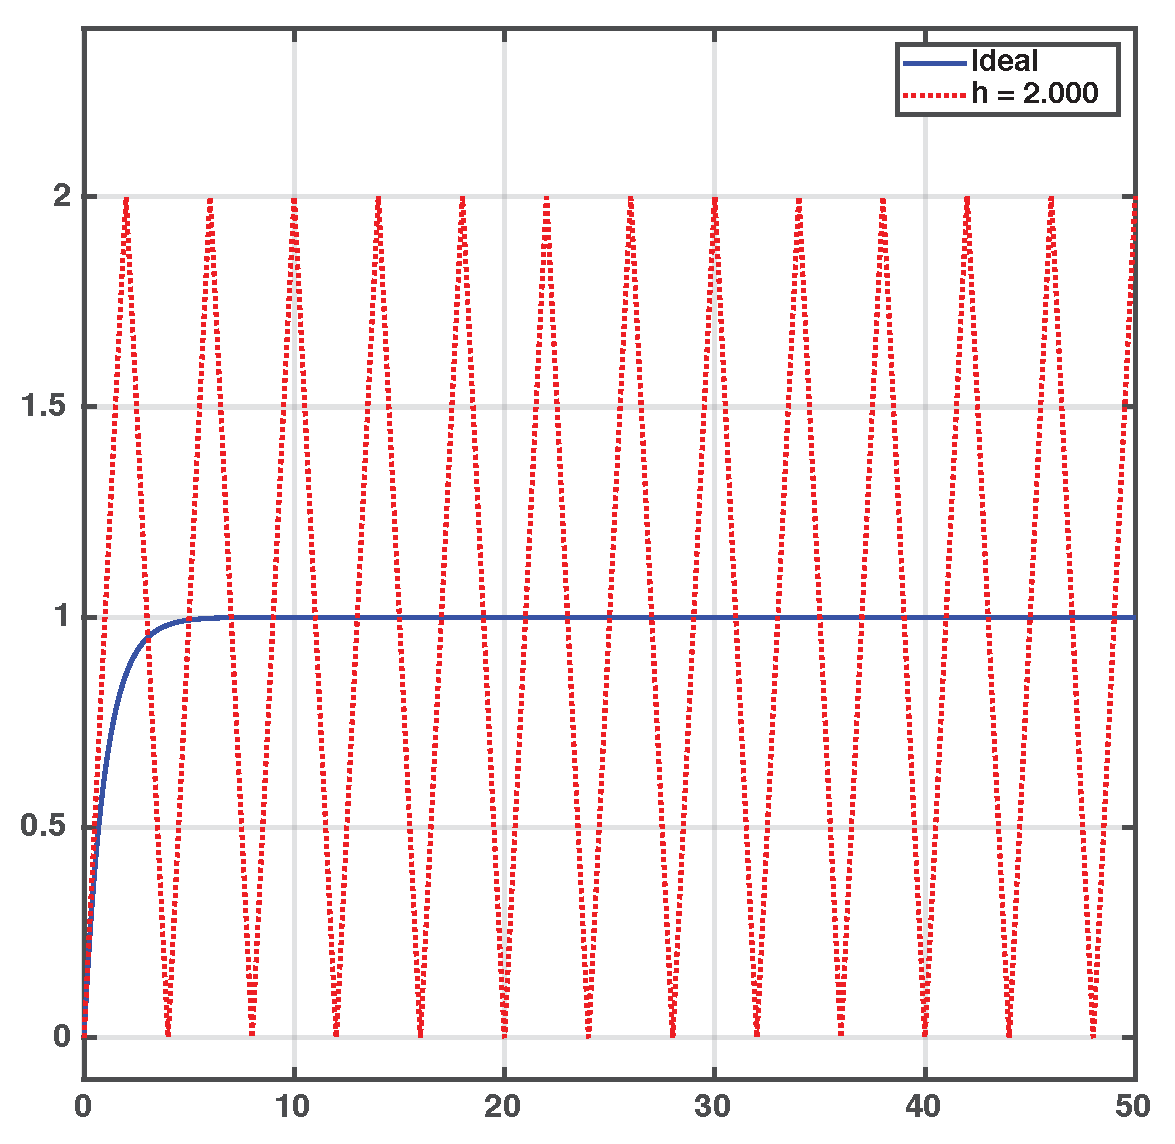
\includegraphics[scale=0.4]{ResearchNotes_TimePDE/figs/forwardOscillations.eps}
\caption{Poor numerical solution with oscillations was obtained as the problem is too stiff for the explicit numerical method.}
\label{fig:falseOscillation}
\end{figure}

Another problem arises when adaptive time stepping is used. As the solution approaches the final steady-state value, the time step will reduce significantly to manage the error within the error tolerance, which leads to long simulation runtime even though the results are converging to the correct solution. These problems can be overcome by implicit methods.

\section{The Backward (Implicit) Euler Method}

As presented in Equation~(\ref{eq:compImEuler}), the implicit Euler method is described by\begin{IEEEeqnarray}{rCl}
y_{n+1} & = & y_{n} + hf(t_{n+1},y_{n+1}) \nonumber
\end{IEEEeqnarray}The solution we are trying to solve for, $y_{n+1}$, appears on both sides of the equation, which makes it cumbersome to solve. The general approach to solve the equation utilizes an educated guess for the solution, $y^{*}_{n+1}$, and a residual function, $R(y^{*}_{n+1})$. If we substitute $y^{*}_{n+1}$ into Equation~(\ref{eq:compImEuler}), we obtain\begin{IEEEeqnarray}{rCl}
y^{*}_{n+1} & = & y_{n} + hf(t_{n+1},y^{*}_{n+1}) + R(y^{*}_{n+1}) \\
R(y^{*}_{n+1}) & = & y^{*}_{n+1} - y_{n} - hf(t_{n+1},y^{*}_{n+1}) \label{eq:imEulerRes}
\end{IEEEeqnarray}We clearly see in Equation~(\ref{eq:imEulerRes}) that $R(y^{*}_{n+1})$ is the error in Equation~(\ref{eq:compImEuler}) if the educated guess was used as the solution. The objective now is to search for $y^{*}_{n+1}$ so that $R(y^{*}_{n+1})=0$. This can be achieved using the Newton-Raphson method. We start by assuming $R(y^{*}_{n+1})$ is sufficiently small that\begin{IEEEeqnarray}{rCl}
R'(y^{*}_{n+1}) & \approx & \frac{R(y^{*}_{n+1})}{y^{*}_{n+1} - y^{**}_{n+1}}
\end{IEEEeqnarray}where $R'(y^{*}_{n+1})$ is the derivative of the residual function with respect to $y^{*}_{n+1}$, and $y^{**}_{n+1}$ is our updated guess of $y_{n+1}$. Rearranging the terms, we obtain the equation\begin{IEEEeqnarray}{rCl}
y^{**}_{n+1} & = & y^{*}_{n+1} - \frac{R(y^{*}_{n+1})}{R'(y^{*}_{n+1})} \label{eq:newtonUpdate0}
\end{IEEEeqnarray}We may then check $(y^{**}_{n+1} - y^{*}_{n+1})$ (and possibly $R(y^{**}_{n+1})$) against some convergence criteria. If the criteria is met, $y^{**}_{n+1}$ is accepted as $y_{n+1}$ and we move to calculate the next time step in the implicit Euler method. If the criteria is not met, we substitute $y^{**}_{n+1}$ as $y^{*}_{n+1}$ in Equation~(\ref{eq:newtonUpdate0}) and update our guess for $y_{n+1}$ to check against the convergence criteria, repeating until the convergence criteria is met.

In many engineering problems, Equation~(\ref{eq:compImEuler}) describes a system of equations where $y_{n+1}$ and $y_{n}$ describes values over a spatial grid at a particular time. In many cases, $f()$ is a matrix describing an operator. Consider the 1-D diffusion equation over a uniform spatial grid on the Cartesian axes described by\begin{IEEEeqnarray}{rCl}
\frac{\partial y}{\partial t} & = & -D\overrightarrow{\nabla}^{2}y \\
& = & -\frac{D}{dx^{2}}Ay
\end{IEEEeqnarray}where $D$is the diffusion coefficient, $dx$ is the spacing between grid points, and $A$ is the tridiagonal matrix representing the Laplacian operator in Cartesian coordinates. Substituting into Equation~(\ref{eq:compImEuler}), the discretized diffusion IVP is solved by the implicit Euler method by\begin{IEEEeqnarray}{rCl}
y_{n+1} & = & y_{n} - h\frac{D}{dx^{2}}Ay_{n+1} \\
\left(I + h\frac{D}{dx^{2}}A\right)y_{n+1} & = & y_{n} \\
y_{n+1} & = & \left(I + h\frac{D}{dx^{2}}A\right)^{-1}y_{n} \label{eq:imEulerDiff}
\end{IEEEeqnarray}where $I$ is the identity matrix. Equation~(\ref{eq:imEulerDiff}) shows that $y_{n+1}$ is found by inverting the matrix $\left(I + h\frac{D}{dx^{2}}A\right)$ and pre-multiplying with $y_{n}$.

\section{Higher Order Implicit Methods}

Just as for explicit methods, a family of higher order implicit methods also exist.

\subsection{The Theta Method}

The Theta method combines the explicit Euler step with an implicit Euler step:\begin{IEEEeqnarray}{rCl}
y_{n+1} & =  y_{n} + h\theta{}f(t_{n},y_{n}) + h(1-\theta)f(t_{n}, y_{n+1})
\end{IEEEeqnarray}The Crank-Nicolson or trapezoidal method is obtained if $\theta=0.5$, and hence\begin{IEEEeqnarray}{rCl}
y_{n+1} & =  y_{n} + h\frac{f(t_{n},y_{n}) + f(t_{n}, y_{n+1})}{2}
\end{IEEEeqnarray}Note that due to the implicit nature of the backward Euler step, the Crank-Nicolson method is not an average between the forward and backward Euler steps. Applying the Crank-Nicolson method to the diffusion IVP as before, we obtain\begin{IEEEeqnarray}{rCl}
y_{n+1} & = & y_{n} - \frac{h}{2}\frac{D}{dx^{2}}Ay_{n} - \frac{h}{2}\frac{D}{dx^{2}}Ay_{n+1} \\
\left(I + \frac{h}{2}\frac{D}{dx^{2}}A\right)y_{n+1} & = & \left(I - \frac{h}{2}\frac{D}{dx^{2}}A\right)y_{n} \\
y_{n+1} & = & \left(I + \frac{h}{2}\frac{D}{dx^{2}}A\right)^{-1}\left(I - \frac{h}{2}\frac{D}{dx^{2}}A\right)y_{n}
\end{IEEEeqnarray}